%%%%%%%%%%%%%%%%%%%%%%%%%%%%%%%%%%%%%%%%%%%%%%%%%%%%%%%%%%%%%%%%%%%%%%%%%%%%%%%%
%2345678901234567890123456789012345678901234567890123456789012345678901234567890
%        1         2         3         4         5         6         7         8

\documentclass[letterpaper, 10 pt, conference]{ieeeconf}  % Comment this line out
                                                          % if you need a4paper
%\documentclass[a4paper, 10pt, conference]{ieeeconf}      % Use this line for a4
                                                          % paper

\IEEEoverridecommandlockouts                              % This command is only
                                                          % needed if you want to
                                                          % use the \thanks command
\overrideIEEEmargins
% See the \addtolength command later in the file to balance the column lengths
% on the last page of the document

\usepackage[utf8]{inputenc}
\usepackage[T1]{fontenc}
\usepackage{graphicx}

% The following packages can be found on http:\\www.ctan.org
%\usepackage{graphics} % for pdf, bitmapped graphics files
%\usepackage{epsfig} % for postscript graphics files
%\usepackage{mathptmx} % assumes new font selection scheme installed
%\usepackage{mathptmx} % assumes new font selection scheme installed
%\usepackage{amsmath} % assumes amsmath package installed
%\usepackage{amssymb}  % assumes amsmath package installed

\title{\LARGE \bf
Penggunaan Unstructured Text dalam Memprediksi Perilaku Pemilih Pemula Pada Pemilihan Calon Legislatif DPR RI Dapil II Jawa Timur 2019
}

%\author{ \parbox{3 in}{\centering Huibert Kwakernaak*
%         \thanks{*Use the $\backslash$thanks command to put information here}\\
%         Faculty of Electrical Engineering, Mathematics and Computer Science\\
%         University of Twente\\
%         7500 AE Enschede, The Netherlands\\
%         {\tt\small h.kwakernaak@autsubmit.com}}
%         \hspace*{ 0.5 in}
%         \parbox{3 in}{ \centering Pradeep Misra**
%         \thanks{**The footnote marks may be inserted manually}\\
%        Department of Electrical Engineering \\
%         Wright State University\\
%         Dayton, OH 45435, USA\\
%         {\tt\small pmisra@cs.wright.edu}}
%}

\author{Risad Tristanto$^{1}$% 
% stops a space
\thanks{*Paper dibuat untuk keperluan studi}% <-this % stops a space
\thanks{$^{1}$Magister Ilmu Komputer,
        Universitas Gadjah Mada, Yogyakarta
        {\tt\small DHLBdatalab.net}}%
}


\begin{document}



\maketitle
\thispagestyle{empty}
\pagestyle{empty}


%%%%%%%%%%%%%%%%%%%%%%%%%%%%%%%%%%%%%%%%%%%%%%%%%%%%%%%%%%%%%%%%%%%%%%%%%%%%%%%%
\begin{abstract}

Tinjauan sistematis ini bertujuan untuk menilai bagaimana informasi dari unstructured text digunakan untuk mengembangkan dan memvalidasi model prediksi perilaku pemilih pemula pada pemilihan Calon Legislatif DPR RI Dapil II Jawa Timur Tahun 2019. Kami merangkum prediksi dan lanskap masalah metodologis dan menentukan apakah penggunaan data teks selain data terstruktur yang lebih umum digunakan akan meningkatkan kinerja prediktif.

\end{abstract}


%%%%%%%%%%%%%%%%%%%%%%%%%%%%%%%%%%%%%%%%%%%%%%%%%%%%%%%%%%%%%%%%%%%%%%%%%%%%%%%%
\section{INTRODUCTION}

Amanat dalam Undang-Undang No. 23 Tahun 20I4 tentang pemerintahan Daerah, ditegaskan bahwa pemilihan kepala daerah dan wakil kepala daerah dipilih secara langsung. Undang-Undang No. l0 Tahun 2008 tentang pemilihan umum disebutkan bahwa pemilih pemula adalah mereka yang baru pertama kali untuk memilih dan telah berusia 17 tahun atau lebih atau sudah pernah menikah mempunyai hak memilih dalam pemilihan umum (dan Pemilukada). Layaknya sebagai pemilih pemula, mereka selalu dianggap tidak memiliki pengalaman memilih (voting pada pemilu sebelumnya). Namun, ketiadaan pengalaman bukan berarti mencerminkan keterbatasan untuk menyalurkan aspirasi politiknya, namun mereka tetap melaksanakan hak pilihnya di tempat pemungutan suara.

Pemilih pemula adalah pemilih yang ikut andil menentukan pemimpin di daerah tertentu. Perilaku pemilih pemula menjadi indikator kualitas demokrasi secara substansial pada saat ini dan masa akan datang. Karena kondisinya masih labil dan mudah dipengaruhi oleh kalangan-kalangan partai politik. Untuk melihat perilaku pemilih pemula ada beberapa pendekatan yang dilihat menurut Dennis Kavanagh melalui buku-nya yang berjudul Political Science and Political Behavior, menyatakan terdapat tiga model untuk menganalisis perilaku pemilih. Yakni pendekatan sosiologis, psikologi sosial, dan pilihan rasional.Ketiga pendekatan tersebut merupakan suatu hal yang fenomenal dan menjadi perilaku memilih masyarakat dalam pemilukada, khususnya dikalangan pemilih pemula yang menjadi dasar dalam menentukan tindakan politiknya. Sehingga pendekatan ini dapat menjelaskan sebab dan arah perilaku pemilih pemula yang akan dibuktikan melalui penelitian ini. Fakta-fakta empirik tersebut yang juga didukung oleh aspek teoritik maka sangat menarik untuk mencermati kecenderungan perilaku politik pemilih pemula dalam menjatuhkan pilihannya kepada seorang calon atau kandidat tertentu di DKI Jakarta pada Tahun 2024.

Penelitian yang selama ini dilakukan adalah dengan melakukan survey secara langsung dengan memberikan pertanyaan-pertanyaan terstruktur untuk mengidentifikasi kecenderungan pilihan. Survey dilakukan dengan 2 cara, online dan offline. Meningkatnya ketersediaan teks tidak terstruktur dalam data survey, peningkatan daya komputasi, dan kemajuan dalam teknik Natural Language Processing (NLP) sekarang memungkinkan penggunaan data teks untuk pengembangan model prediksi. Akibatnya, tujuan dari tinjauan ini adalah untuk menilai bagaimana informasi yang diekstraksi dari teks tidak terstruktur dalam data survey digunakan untuk mengembangkan dan memvalidasi model prediksi perilaku pemilih pemula. Kami mengevaluasi studi tentang pengaturan dan populasi studi, metode dan representasi pemrosesan teks, metode pembelajaran mesin dan kombinasi set fitur, evaluasi kinerja dan validasi eksternal, perhatian pada keterjelasan model, dan ketersediaan model. Selanjutnya, kami menentukan nilai teks selain data terstruktur dengan membandingkan kinerja antara model menggunakan set fitur yang berbeda dalam studi.


\section{BAHAN DAN MATERI}

\subsection{Tinjauan Konseptual}

Jumlah penduduk sebanyak 38.369 jiwa, penduduk yang kategori pemilih pemula adalah sebanyak 3.724 jiwa yaitu antara usia 15-19 tahun. Berdasarkan Undang-Undang Nomor 10 Tahun 2008, pada Pasal 1 ayat (22), pemilih pemula adalah penduduk yang sudah berusia 17 tahun keatas. Pemilih yang sudah menikah. Berarti usia 15 dan 16 tahun dapat diwajibkan untuk memilih asalkan sudah menikah.

Berdasarkan data yang diperoleh dari KPU Kecamatan Pandaan. Bahwa penduduk yang berusia 15 sampai 17 tahun serjumlah sebanyak 373 jiwa, yaitu sebesar 10 persen dari total jumlah penduduk Kecamatan Pandaan. Dari 373 jiwa yang berhak memilih usia 15-16 tahun yang sudah menikah sebanyak 60 jiwa, sedangkan sisanya sebanyak 313 jiwa yang berusia 17 tahun

\subsection{Pengumpulan Data}

Dalam hal ini peneliti melakukan sampel dengan menyebar kuisioner dengan melakukan 3 (tiga) pendekatan yaitu pendekatan sosiologis, dan pendekatan hirtoris, serta pendekatan rasional.Dimana untuk pendekatan sosiologis dan historis peneliti gabungkan jumlah responden, dimana pendekatan sosiologis sebanyak 39 responden, sedangkan pendekatan historis sebanyak 2l responden.

\begin{figure}
\centering
\fbox{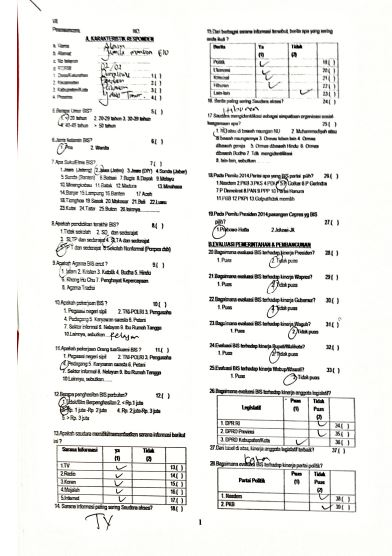
\includegraphics[width=\linewidth]{kues 1.JPG}}
\caption{Contoh hasil kuesioner}
\label{fig:false-color}
\end{figure}

\subsection{Metode Penelitian}

Pendekatan penelitian yang digunakan adalah pendekatan kualitatif dan kuantitatif dengan pola 2 (dua) tahap, sejalan dengan metoda yang digunakan, yakni metoda studi kasus. Alasan pemilihan studi kasus adalah sebagaimana dijelaskan oleh Merriam, Yin dalam Cresswell (1994:12), bahwa:

Case studies, in which the researcher explores a single entity or phenomenon ("the case") bounded by time and activity (a program, event, process, institution, or social group) and collects detailed information by using a variety of data collection procedure during a sustained period of time.

Melalui studi kasus diharapkan model yang dihasilkan pada Kabupaten/Kota lokasi penelitian akan dapat direpresentasikan atau digunakan untuk menggambarkan dan menjelaskan kasus-kasus serupa di Kabupaten/Kota lain.

\section{HASIL DAN PEMBAHASAN}

Untuk melihat perilaku pemilih pemula ada beberapa pendekatan yang dilihat menurut Dennis Kavanagh melalui buku-nya yang berjudul Political Science and Political Behavior, menyatakan terdapat tiga model untuk menganalisis perilaku pemilih, yakni pendekatan sosiologis, psikologi sosial, dan pilihan rasional. Merujuk pada hasil studi serta pendekatan-pendekatan di atas, penelitian ini mencoba menggambarkan dan menganalisis tentang kecenderungan perilaku pemilih pemula. Degan ketiga pendekatan ini, peneliti telah mendapatkan data sample pada lembar data survey yang selanjutnya akan dianalisis untuk melihat kecenderungan perilaku pemilih pemula dengan melakukan ekstraksi dari unstructured data pada lembaran survey untuk ditemukan sebuah model prediktif baru.


\subsection{Ekstraksi dan Sintesis Data} 

Data untuk analisis diekstraksi dari studi yang dilakukan sebelumnya melalui survey dengan 3 pendekatan seperti yang telah dijelaskan sebelumnya menggunakan set item data yang telah ditentukan sebelumnya, diuraikan dalam Tabel 1.

Input untuk metode text representation terdiri dari representasi vektor numerik yang jarang (sparse) dan padat (dense). Sparse representation terdiri dari data hasil survey yang terdiri dari beberapa subjek penelitian serta beberapa poin tambahan yang berkaitan dengan perilaku individu maupun kelompok serta pengaruh lingkungan terhadap perilaku pemilih pemula dalam menentukan pilihannya. sedangkan dense representation terdiri dari model topik, penyisipan kata dan dokumen, dan skor ringkasan, seperti skor sentimen. Metode machine learning memiliki kompleksitas dan interpretasi yang bervariasi, mulai dari metode dengan kompleksitas yang relatif rendah dan interpretasi yang tinggi, seperti regresi linier atau logistik, hingga random forests yang semakin kompleks, peningkatan gradien dan Support Vector Machine (SVM).

\begin{table}[h]
\caption{Daftar item data untuk ekstraksi data, berdasarkan topik}
\label{table_example}
\begin{center}
\begin{tabular}{|c||c||c|}
\hline
Item Topic & Data Item & Tipe Input\\
\hline
Karakteristik Responden & Nama & Free text\\
\hline
 & Alamat & Free text\\
\hline
 & No. Telpon & Number\\
\hline
 & RT/RW & Free text\\
\hline
 & Desa/Kelurahan & Free text\\
\hline
 & Kecamatan & Free text\\
\hline
 & Kabupaten/Kota & Free text\\
\hline
 & Propinsi & Free text\\
\hline
& Umur & Option Number\\
\hline
& Jenis Kelamin & Option Number\\
\hline
& Suku & Option Number\\
\hline
& Pendidikan & Option Number\\
\hline
& Agama & Option Number\\
\hline
& Pekerjaan & Option Number\\
\hline
& Pekerjaan Orang Tua/Pasangan & Option Number\\
\hline
& Penghasilan & Option Number\\
\hline
& Memiliki TV & Yes or No\\
\hline
& Memiliki Radio & Yes or No\\
\hline
& Memiliki Koran & Yes or No\\
\hline
& Memiliki Majalah & Yes or No\\
\hline
& Memiliki Internet & Yes or No\\
\hline
& Media paling sering diakses & Free text\\
\hline
& Mengikuti berita politik & Yes or No\\
\hline
& Mengikuti berita ekonomi & Yes or No\\
\hline
& Mengikuti berita kriminal & Yes or No\\
\hline
& Mengikuti berita hiburan & Yes or No\\
\hline
& Mengikuti berita lainnya & Yes or No\\
\hline
& Berita paling sering diikuti & Free text\\
\hline
& Keanggotaan Ormas & Option Number\\
\hline
& Pilihan Partai Politik 2014 & Option Number\\
\hline
& Pilihan Capres/Cawapres 2014 & Option Number\\
\hline
Evaluasi Pemerintahan & Puas Kinerja Presiden & Yes or No\\
\hline
 & Puas Kinerja Wakil Presiden & Yes or No\\
\hline
 & Puas Kinerja Gubernur & Yes or No\\
\hline
 & Puas Kinerja Wakil Gubernur & Yes or No\\
\hline
 & Puas Kinerja Bupati/Walikota & Yes or No\\
\hline
 & Puas Kinerja Wakil Bupati/Walikota & Yes or No\\
\hline
 & Puas Kinerja DPR RI & Yes or No\\
\hline
 & Puas Kinerja DPRD Propinsi & Yes or No\\
\hline
 & Puas Kinerja DPRD Kabupaten/Kota & Yes or No\\
\hline
 & Kinerja legislatif terbaik & Free text\\
\hline
\end{tabular}
\end{center}
\end{table}






\end{document}
